

% LaTeX file for Chapter Exp2






\chapter{Experiment 2: ITE on International Stroke Trial (IST)} \label{ch:exp2}





\section{Motivation}


% describe the data of stroke trial https://pubmed.ncbi.nlm.nih.gov/9174558/
% Results on IST trial with the interpretation in the discussion part.

%  here the authors made the IST database available and described the trial, we downloaded the CSV
% https://trialsjournal.biomedcentral.com/articles/10.1186/1745-6215-12-101 


% Results: The IST dataset includes data on 19 435 patients with acute stroke, with 99% complete follow-up. Over 26.4% patients were aged over 80 years at study entry. Background stroke care was limited and none of the patients received thrombolytic therapy.
% 
% 
\citet{chen2025} evaluated multiple causal ML methods on the International Stroke Trial (IST), to estimate the individualized treatment effects. They demonstrated that none of the applied ML methods generalized well, as performance on the test data differed significantly from the training data on the chosen evaluation metrics.
In this experiment, we replicate the analysis on the same data by applying three causal ML methods for ITE estimation, to investigate whether we obtain similar results as the authors.


\section{Setup} \label{sec:methods_experiment2}



\textbf{Data:} The International Stroke Trial was a large, randomized controlled trial conducted in the 1990s to assess the efficacy and safety of early antithrombotic treatment in patients with acute ischemic stroke \citep{IST1997}. Using a 2x2 factorial design, 19,435 patients across 36 countries were randomized within 48 hours of symptom onset to receive aspirin, subcutaneous heparin, both, or neither. Patients allocated to aspirin (300 mg daily for 14 days) had a 6-month death or dependency rate of 62.2\%, compared to 63.5\% in the control group not receiving aspirin, corresponding to a statistically significant absolute risk reduction after adjustment for baseline prognosis (1.4\%, p = 0.03). The authors stated that there was no interaction between aspirin and heparin in the main outcomes. In this thesis, we focus exclusively on the aspirin vs. no aspirin comparison and the outcome of death or dependency at 6 months after stroke.

The dataset used in this experiment was made publicly available by \citet{sandercock2011} and contains individual-level data, including baseline covariates assessed at randomization, treatment allocation, and 6-month outcomes, with a follow-up rate of 99\%.

We used the same data pre-processing steps as \citet{chen2025} to ensure comparability of results. 5.9\% of individuals had incomplete data and were removed from the dataset. We used 2/3 of the data for fitting the models and 1/3 as a hold out test set. The final dataset included 21 baseline variables recorded at randomization: aspirin allocation (treatment), age, delay between stroke and randomization (in hours), systolic blood pressure, sex, CT performed before randomization, visible infarct on CT, atrial fibrillation, aspirin use within 3 days prior to randomization, and presence or absence of neurological deficits (including face, arm/hand, leg/foot deficits, dysphasia, hemianopia, visuospatial disorder, brainstem or cerebellar signs, and other neurological deficits), as well as consciousness level, stroke subtype, and geographical region. The outcome variable was death or dependence at 6 months.


\medskip

\textbf{Models for ITE estimation: } The aim is to estimate the ITE based on baseline characteristics. As a benchmark, we apply a T-learner logistic regression (following \citet{chen2025}, using the \texttt{stats} package). As a more complex model, we apply a T-learner tuned random forest (using the \texttt{comets} package \citep{comets}), which tunes the number of variables considered for splitting at each node (\texttt{mtry}) and the maximum tree depth (\texttt{max.depth}) using out-of-bag error, with 500 trees. Additionally, we apply an S-learner TRAM-DAG. For the random forest and TRAM-DAG based methods, we additionally scale numerical and dummy encode categorical covariates prior to model training. The transformation function of the outcome is modelled by a complex intercept $h(Y \mid T, \mathbf{X}) = CI(T, \mathbf{X})$, with 4 hidden layers of shape (20, 10, 10, 2). This architecture allows for interaction between the treatment and covariates. Furthermore, batch normalization, ReLU activation, and dropout (0.1) are applied to prevent overfitting and stabilize learning. A validation set comprising 20\% of the training data is used to select the model with the lowest out-of-sample negative log-likelihood, while the test set remains untouched for final evaluation. 

Since the IST is a randomized controlled trial, the full potential of TRAM-DAGs -- designed primarily for use in observational settings -- is not required here, as only the outcome needs to be modeled as a function of baseline patient characteristics. However, applying TRAM-DAGs in this context still allows us to assess its predictive performance and ability to flexibly model interactions between variables.



\medskip

\textbf{Model evaluation: } For validation, since the ground truth is not known, we first rely on calibration plots to assess the general prediction power for the probabilities. Second, we predict the potential outcomes with the trained models to estimate the ITE on the training and test set in terms of the risk difference $\text{ITE}_i = \text{P}(Y_i=1|T=1, \mathbf{X}_i) - \text{P}(Y_i=1|T=0, \mathbf{X}_i)$. For visual validation, we show the densities of the estimated ITEs on both datasets, and the ITE-ATE plots to assess whether the estimated ITEs align with the observed outcomes.










% possible example of unobserved interaction:
% An example could be the psychological condition of a patient which might also affect how the treatment works, this is not a confounder but an effect modifier, and i would assume that this variable is rarely recorede or measured.




\section{Results} \label{sec:results_experiment2}


In this section, we present the results of the ITE estimation on the International Stroke Trial (IST) dataset. The observed average treatment effect (ATE), defined as $\text{P}(Y=1|T=1) - \text{P}(Y=1|T=0)$, was -2.4\% absolute risk reduction on the training set, with a 95\% confidence interval from -4.1\% to -0.6\%. The interval was computed using the Wald method for risk differences, with standard error $\sqrt{p_1 (1 - p_1)/n_1 + p_0 (1 - p_0)/n_0}$
, where $p_1$ and $p_0$ are the event rates in the treated and control groups. On the test set, the observed treatment effect was -0.1\%, with a 95\% confidence interval from -2.6\% to 2.3\%. The ITEs were estimated using three different models: T-learner logistic regression, T-learner tuned random forest, and S-learner TRAM-DAG. The estimated average treatment effect on the test set, calculated as $\text{ATE}_\text{pred}=\text{mean}(\text{ITE}_\text{pred})$, was -2.5\% for the T-learner logistic regression, -2.2\% for the T-learner tuned random forest, and -3.1\% for the S-learner TRAM-DAG. The density of predicted ITEs and the ITE-ATE plots for risk difference per estimated ITE subgroup, including 95\% confidence intervals, are presented in Figures \ref{fig:IST_density_ITE_ATE_glm_tlearner} - \ref{fig:IST_density_ITE_ATE_TRAM_DAG}. Calibration plots are provided in Appendix \ref{sec:calibrations_experiment2}, Figures \ref{fig:calibration_IST_glm} - \ref{fig:calibration_IST_TRAM_DAG}. 




\begin{figure}[htbp]
\centering
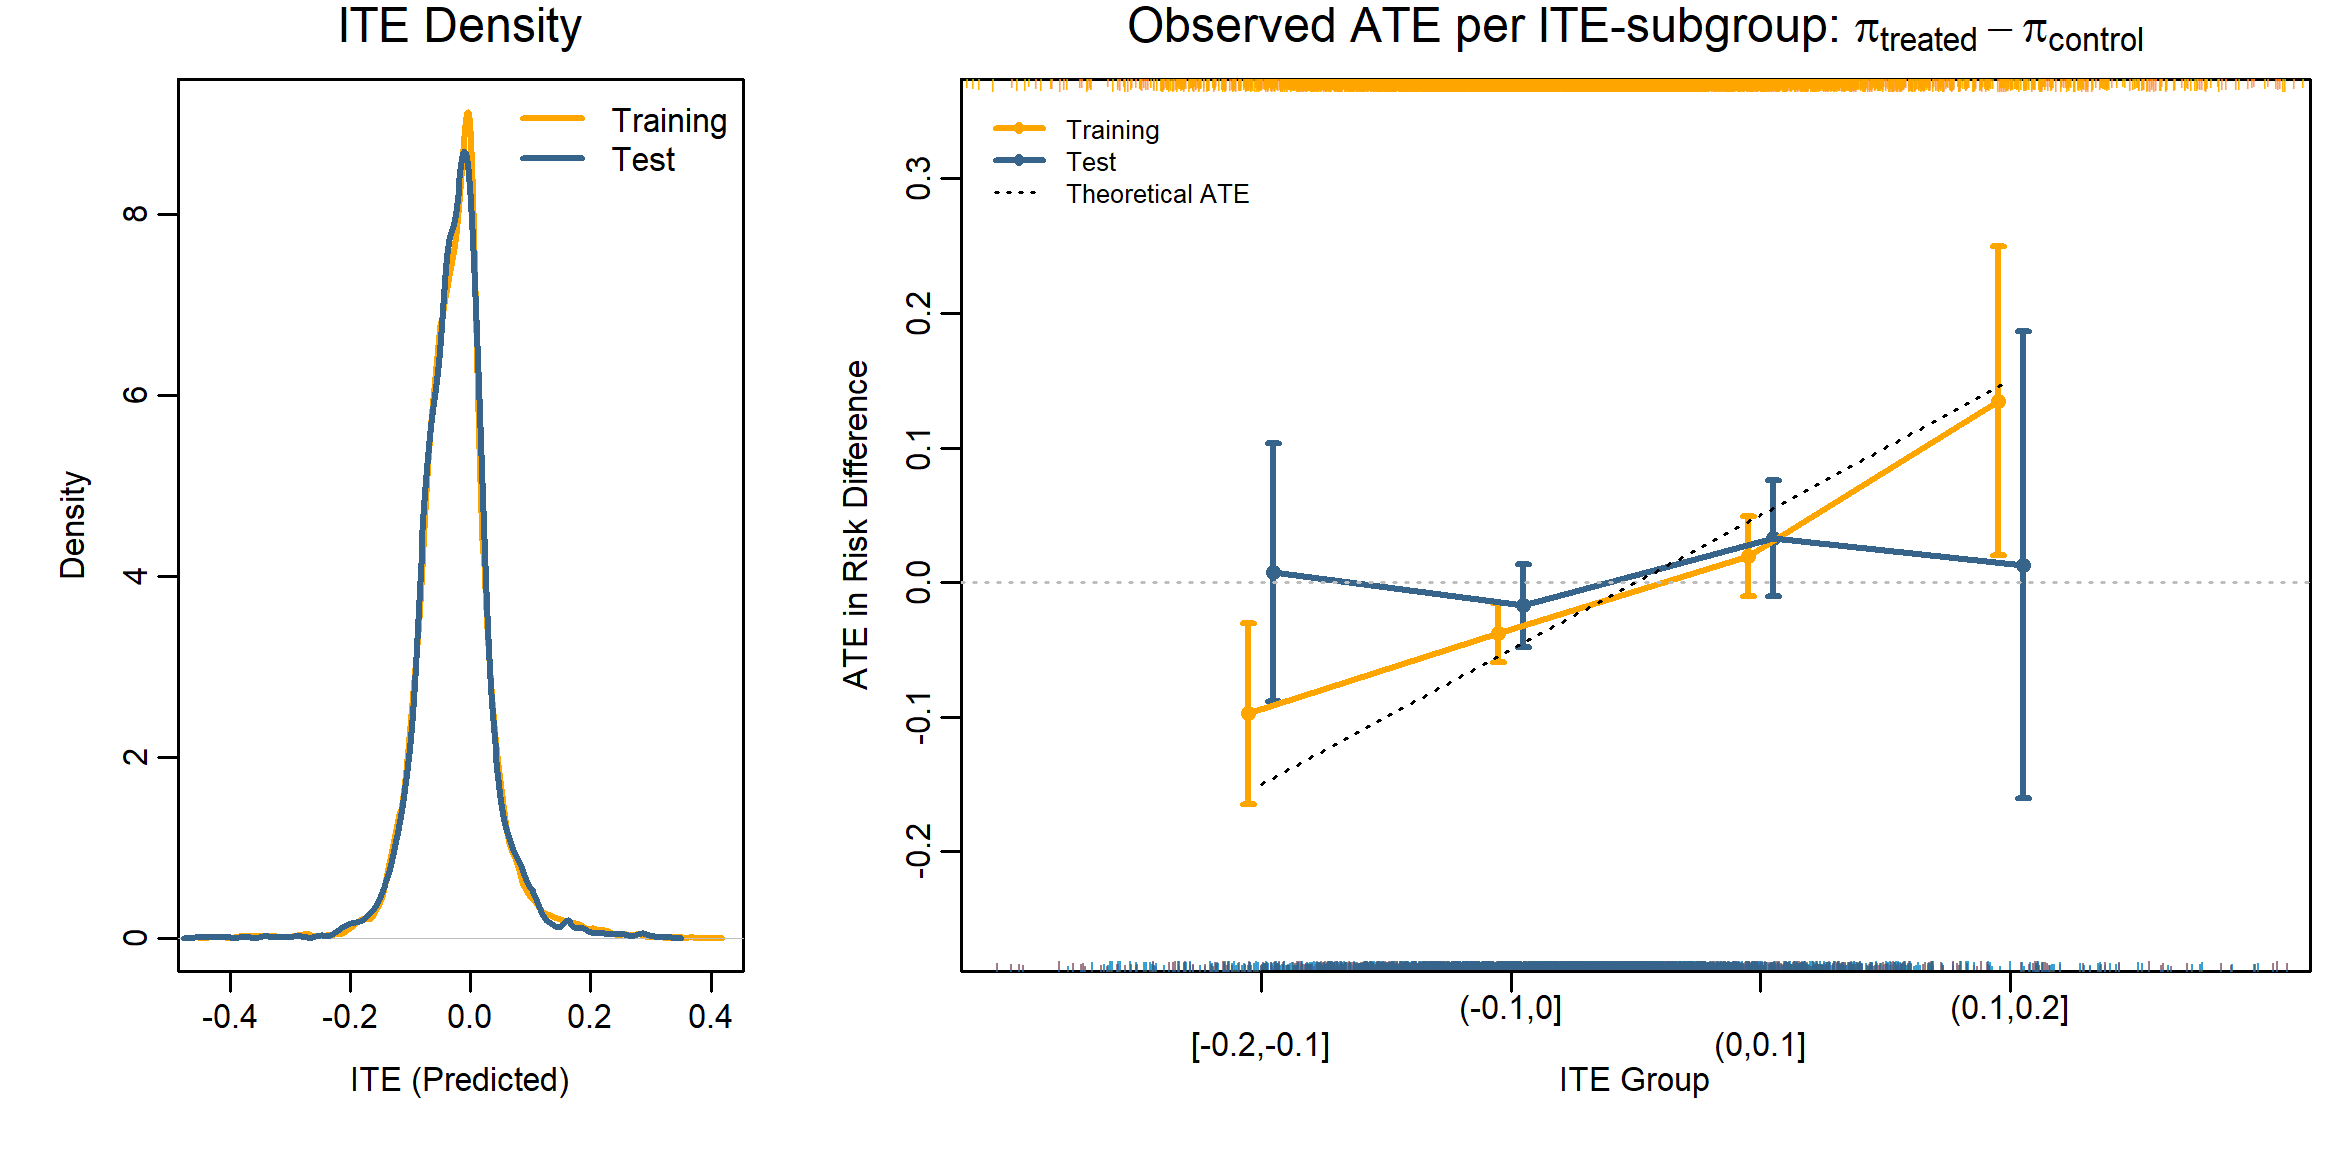
\includegraphics[width=0.9\textwidth]{img/results_IST/glm_tlearner_density_ITE_ATE.png}
\caption{Results for the International Stroke Trial (IST) using the T-learner logistic regression. Left: density of predicted ITEs in the training and test sets; Right: observed ATE in terms of risk difference per estimated ITE subgroup.}
\label{fig:IST_density_ITE_ATE_glm_tlearner}
\end{figure}



\begin{figure}[htbp]
\centering
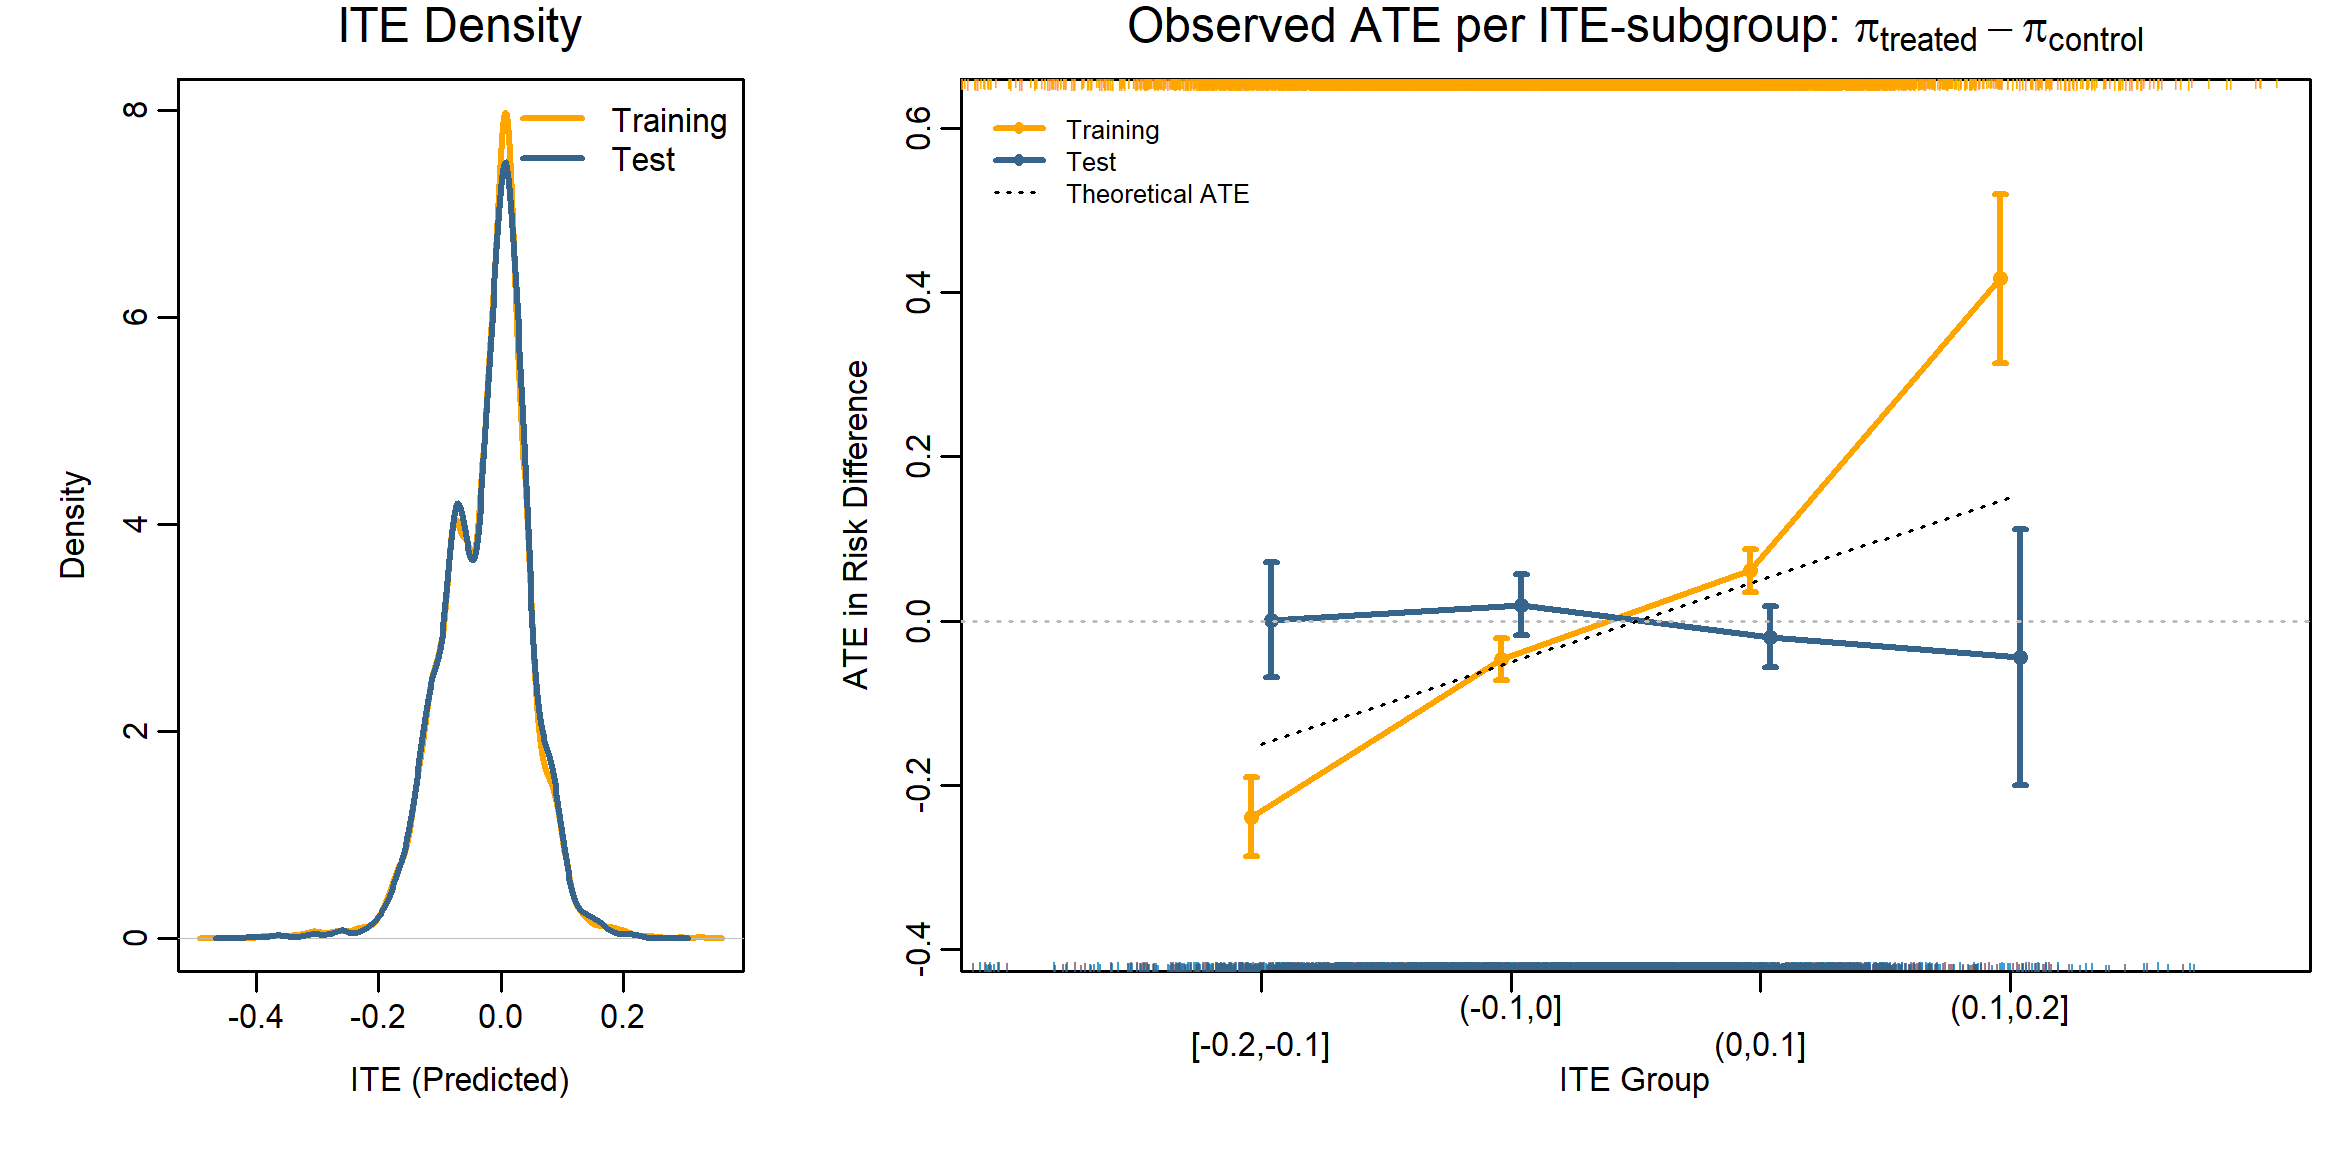
\includegraphics[width=0.9\textwidth]{img/results_IST/IST_tuned_rf_tlearner_density_ITE_ATE.png}
\caption{Results for the International Stroke Trial (IST) using the T-learner tuned random forest. Left: density of predicted ITEs in the training and test sets; Right: observed ATE in terms of risk difference per estimated ITE subgroup.}
\label{fig:IST_density_ITE_ATE_tuned_rf}
\end{figure}


\begin{figure}[htbp]
\centering
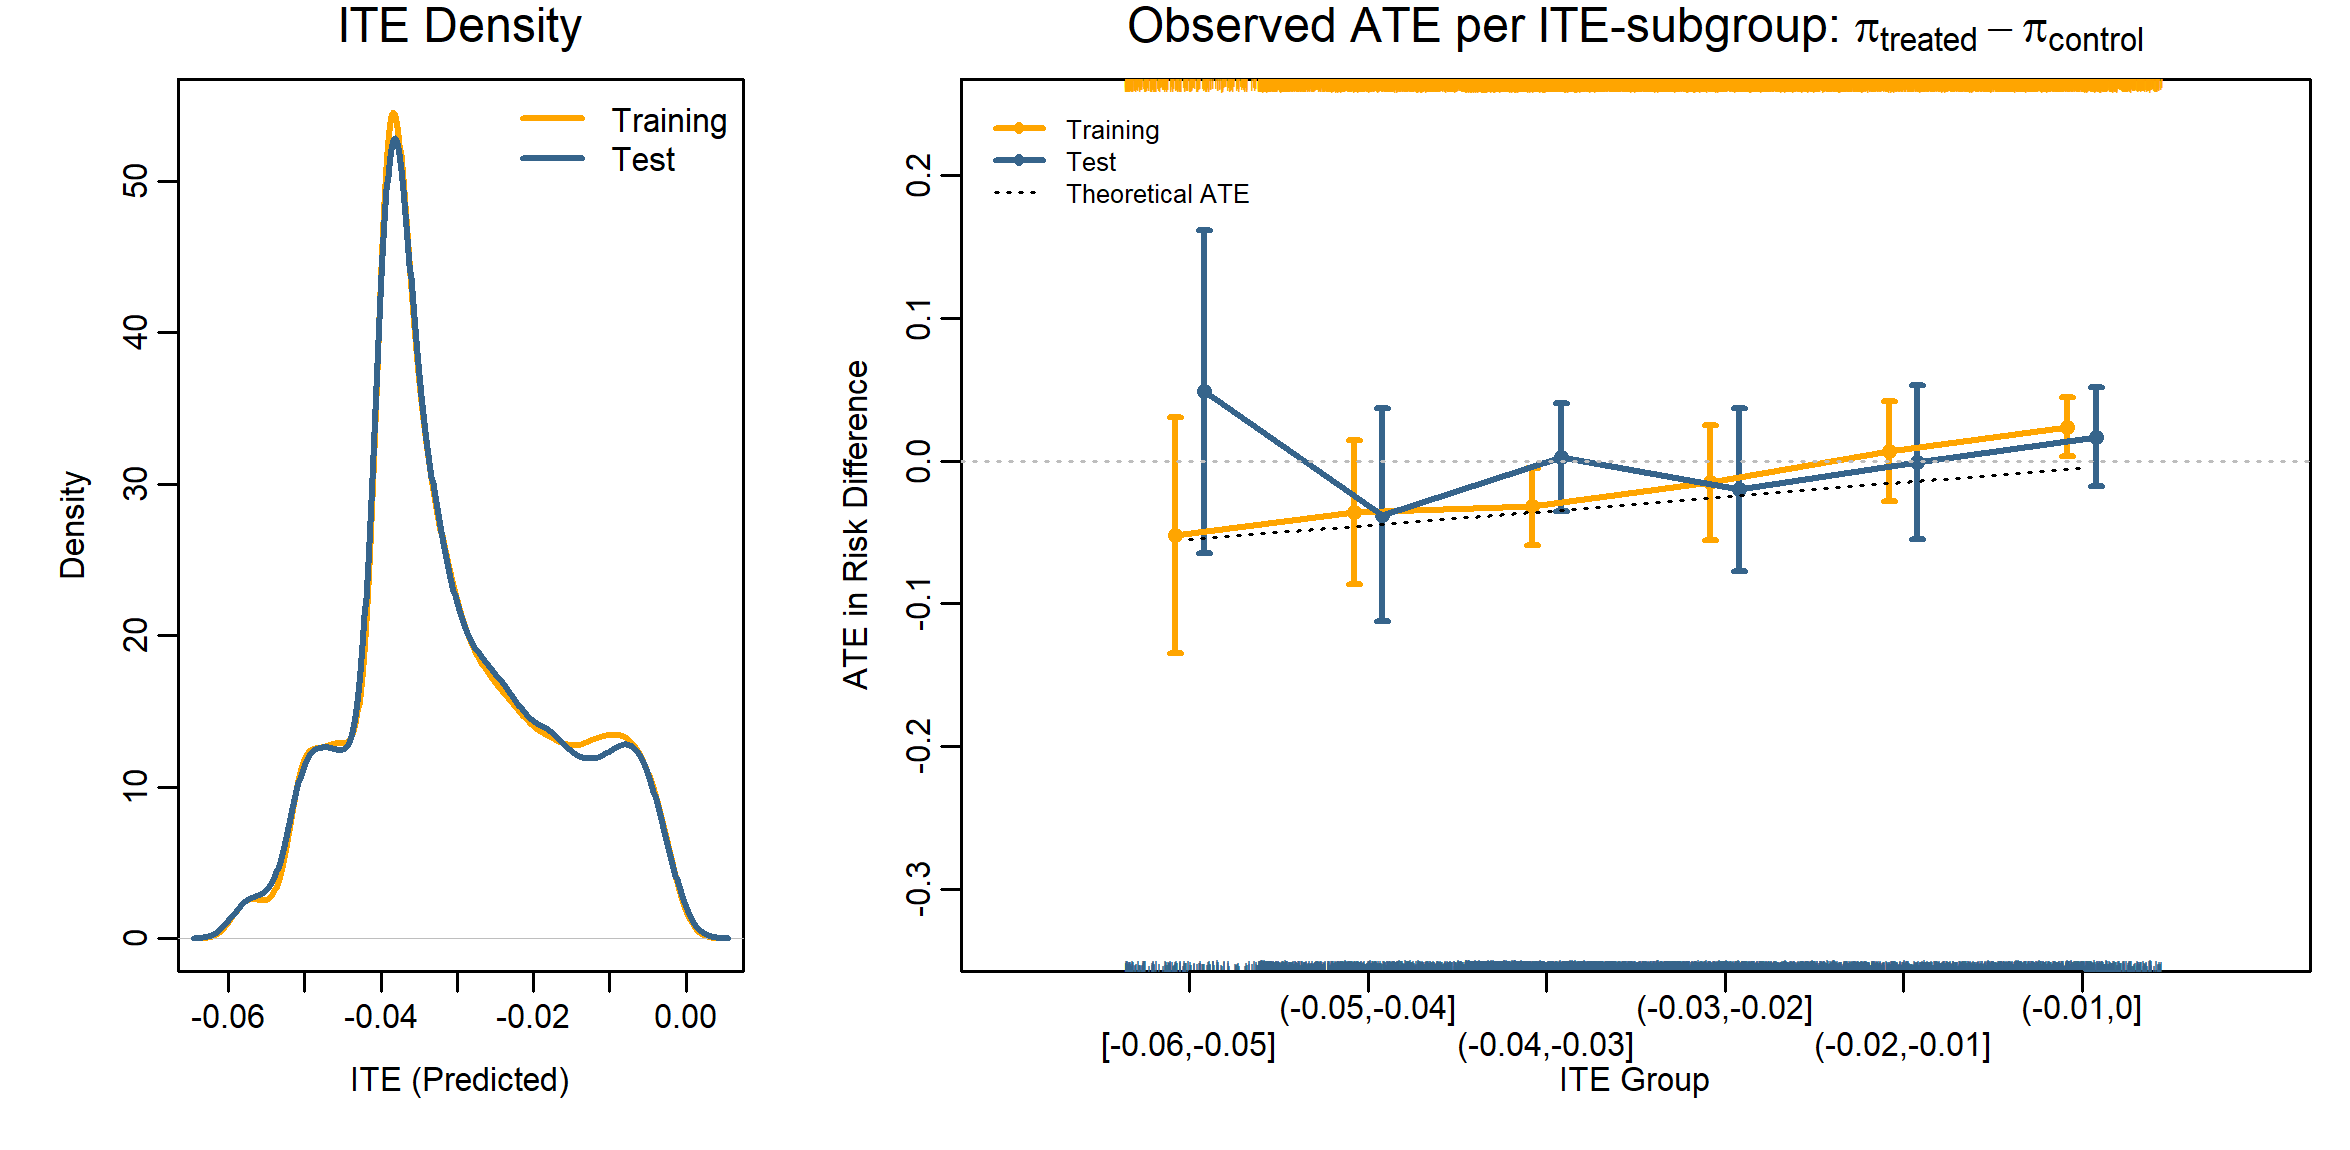
\includegraphics[width=0.9\textwidth]{img/results_IST/IST_TRAM_DAG_slearner_density_ITE_ATE.png}
\caption{Results for the International Stroke Trial (IST) using the S-learner TRAM-DAG. Left: density of predicted ITEs in the training and test sets; Right: observed ATE in terms of risk difference per estimated ITE subgroup.}
\label{fig:IST_density_ITE_ATE_TRAM_DAG}
\end{figure}




% enforce that starts after all floats have been displayed
\FloatBarrier

\section{Discussion}

We observed similar results to those reported by \citet{chen2025} when estimating ITEs on the International Stroke Trial dataset across all three models: the T-learner logistic regression, the T-learner tuned random forest, and the S-learner TRAM-DAG. The logistic model showed moderate discrimination in the training set, which did not generalize to the test set, as illustrated by the ITE-ATE plot in Figure~\ref{fig:IST_density_ITE_ATE_glm_tlearner}. The tuned random forest model showed stronger discrimination in the training set but similarly failed to generalize to the test set (Figure~\ref{fig:IST_density_ITE_ATE_tuned_rf}). In contrast, the S-learner TRAM-DAG estimated less heterogeneity than the other two models, as shown in the density plot in Figure~\ref{fig:IST_density_ITE_ATE_TRAM_DAG}, resulting in weak discrimination in both the training and test sets. For all three models, the confidence intervals in the ITE-ATE plots on the test set included the zero line, suggesting no significant effect in any of the estimated ITE subgroups.

\medskip


Poor calibration does not appear to explain the limited ITE performance, as calibration on the test set was good, as shown in Appendix~\ref{sec:calibrations_experiment2}, Figures~\ref{fig:calibration_IST_glm}-\ref{fig:calibration_IST_TRAM_DAG}. However, since the ground truth is unknown, it remains unclear whether the models fail to detect true treatment effect heterogeneity, or whether the heterogeneity is too small, or driven by unobserved effect modifiers. We investigate these possibilities further in Experiment 3, Chapter~\ref{ch:experiment3}.


